\documentclass[12pt,a4paper]{article}
\usepackage{mathptmx} % added for time new roman font
\usepackage[left=0.5in,right=0.5in,top=1in,bottom=1in]{geometry}
\usepackage[latin1]{inputenc}
\usepackage{amsmath}
\usepackage{amsfonts}
\usepackage{amssymb}
\usepackage{graphicx}
\usepackage{float}
\usepackage{booktabs}
\usepackage{parskip} % remove all the paragraph indents


\usepackage{setspace}
\usepackage[colorlinks=true]{hyperref}
\usepackage{textcomp} 
\usepackage{multicol} 

\usepackage{mathtools}          %loads amsmath as well added for the piece wise function
\DeclarePairedDelimiter\Floor\lfloor\rfloor
\DeclarePairedDelimiter\Ceil\lceil\rceil

 
\newcounter{NumberInTable}
\newcommand{\LTNUM}{\stepcounter{NumberInTable}{(\theNumberInTable)}}

\newcommand{\Laplace}[1]{\ensuremath{\mathcal{L}{\left[#1\right]}}}
\newcommand{\InvLap}[1]{\ensuremath{\mathcal{L}^{-1}{\left[#1\right]}}}
\renewcommand{\textuparrow}{$\uparrow$}

\begin{document}
	
	\large{}
	\title{\vspace{-2cm}Lecture Notes, Topic-9}
	\date{}
	\maketitle
	
	\section*{Review from previous class}
		\begin{enumerate}
			\item Base excitations
		\end{enumerate}
	
	\section*{Objectives for today's class}
	\begin{enumerate}
		\item  Transform Method
	\end{enumerate}
	
	\section*{Lecture}

		\subsection*{Transfer Function method (Generic)}

Consider the following system
\begin{figure}[H]
	\centering
	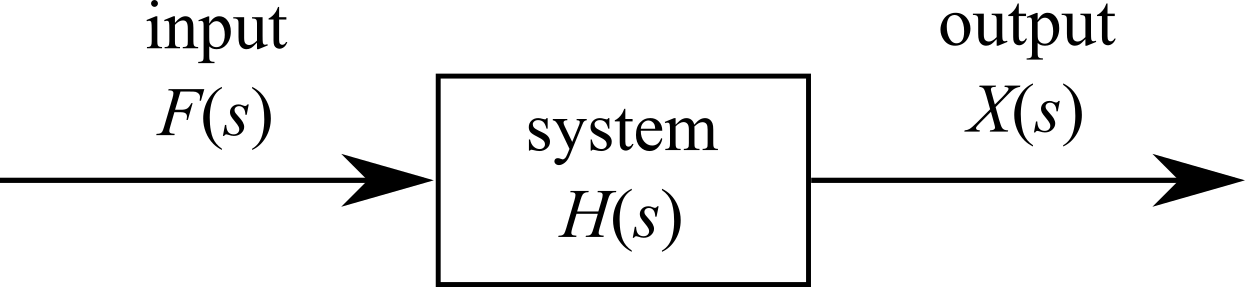
\includegraphics[width=0.5\textwidth]{../../Figures/system_input_output.png}
\end{figure}
where $F(s)$ is the input, $H(s)$ is the system, and $X(s)$ is the output from the system. This formulation is called the transfer-function approach and is commonly used for the formulation and solution of dynamic problems in the control literature. It can also be used for solving the various forced-vibration problems including those from complex or stochastic inputs. 

Examples of force excitation that can be calculated include using this method include:
\begin{itemize}
	\item sinusoidal
	\item base excitation
	\item impulse
	\item arbitrary input
	\item arbitrary periodic input
\end{itemize}

		\subsection*{Review of Laplace Transforms}
		
		 An integral transform is the procedure of integrating the time dependence of a function into becoming a function of an alternative variable, or parameter, which can be manipulated algebraically. 
		
		Of interest to this class is the Laplace transform ($\Laplace{f(t)}$) of the function $f(t)$. Here, a Laplace transform is used as a method of solving the differential equations of motion by reducing the computation needed to that of integration and algebraic manipulation. 
		
		The definition of the Laplace transform of the function $f(t)$ is:
		
		\begin{equation}
				\Laplace{f(t)} = F(s) = \int_{0}^{\infty} f(t)e^{-st}dt
		\end{equation}
		where $f(t)=0$ for all values of $t$ less than 0. Here, the $s$ is a complex value. Lastly, the term $F(s)$is a generic term that  represents the input to a system. As this class needs the derivative of functions, we will calculate that next:
		\begin{equation}
			\Laplace{\dot{f}(t)} = \int_{0}^{\infty} \dot{f}(t)e^{-st}dt = \int_{0}^{\infty} e^{-st}\frac{d[f(t)]}{dt}dt 
		\end{equation}		
		integration by parts yields
		\begin{equation}
			\Laplace{\dot{f}(t)} = e^{-st}f(t)\Big|_0^\infty+s\int_{0}^{\infty}e^{-st}f(t)dt
		\end{equation}
		Astutely, it can be noticed that the second term $s\int_{0}^{\infty}e^{-st}f(t)dt$
		is the input to the system $F(s)$. Therefor, with a little rearranging this becomes:
		\begin{equation}
			\Laplace{\dot{f}(t)} = sF(s)-f(0)
		\end{equation}
		Successive iteration yields:
		\begin{equation}
			\Laplace{\ddot{f}(t)} = s^2F(s)-sf(0)-\dot{f}(0)
		\end{equation}
		
		A few key points of the Laplace transforms are:
		
		
		\begin{itemize}
			\item the domain of the problem from the real number line ($t$) to the complex plane ($s$).
			\item The integration of the Laplace transform changes differentiation into multiplication.
			\item The transform procedure is linear. Therefore, the transform of the linear combination of two transforms is the same as the linear transformation of these functions. 
			\item to move from the time domain to the complex number plane we typically use tables of pre-solved integral. 
			\item The function $x(t)$ can be obtained by taking the inverse Laplace transform defined as $x(t) = \Laplace{X(s)}^{-1}$
		\end{itemize}
		
		The Laplace transform can be calculated in symbolic form. In particular interest to this class is the Laplace form of the system output $X(s)$

		\begin{equation}
			\Laplace{x(t)} = X(s)
		\end{equation}		
		\begin{equation}
			\Laplace{\dot{x}(t)} = sX(s)-x(0)
		\end{equation}	
		\begin{equation}
			\Laplace{\ddot{x}(t)} = s^2X(s)-sx(0) - \dot{x}(0)
		\end{equation}	
		here, $x(0)$ and $\dot{x}(0)$ are the initial values of the function $x(t)$. 
		


The procedure for using the Laplace transform to solve equations of motion expressed as an inhomogeneous ordinary differential equation is:
\begin{enumerate}
	\item Take the Laplace transform of both sides of the EOM while treating the time derivatives symbolically.
	\item Solve for $X(s)$ in the obtained equation.
	\item Apply the inverse transform $x(t) = \Laplace{X(s)}^{-1}$
\end{enumerate}

\subsection*{Transfer Function method (homogeneous differential equation)}

Consider the undamped single-DOF system:
\begin{figure}[H]
	\centering
	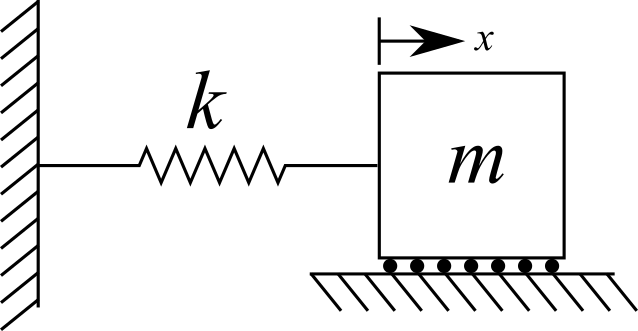
\includegraphics[width=0.4\textwidth]{../../Figures/1-DOF-mass_horizontal.png}
\end{figure}
that can be described the the EOM in standard form:
\begin{equation}
	\ddot{x}(t) + \omega_n^2x(t) = 0 
\end{equation}
where the initial conditions are $x(0)=x_0$ and $\dot{x}(0) = v_0$. Taking the Laplace transforms of both sides of the EOM yields:
\begin{equation}
	\ddot{x}(t)  = s^2X(s) -sx_0 -v_0
\end{equation}
\begin{equation}
	\omega_n^2x(t) = \omega_n^2X(s)
\end{equation}
resulting in:
\begin{equation}
	s^2X(s) -sx_0 -v_0 + \omega_n^2X(s) = 0
\end{equation}
solving for the output of the system $X(s)$ yields:
\begin{equation}
X(s) = \frac{sx_0 + v_0}{s^2 + \omega_n^2}
\end{equation}
We can expand this form of $X(s)$ to obtain equations listed in our Laplace Transform table:
\begin{equation}
X(s) = \frac{sx_0}{s^2 + \omega_n^2} + \frac{v_0}{s^2 + \omega_n^2}\cdot \frac{\omega_n}{\omega_n}
\end{equation}
This becomes:
\begin{equation}
X(s) = x_0\frac{s}{s^2 + \omega_n^2} + \bigg(\frac{v_0}{\omega_n}\bigg) \cdot \frac{\omega_n}{s^2 + \omega_n^2}\cdot 
\end{equation}

Next, using the inverse Laplace transform $x(t) = \Laplace{X(s)}^{-1}]$ and the two following Laplace transforms (\#5 and \#6):
\begin{equation}
f(t) \text{ is cos}(\omega t) \text{ when }  F(s) \text{ is } \frac{s}{s^2+\omega^2} 
\end{equation}
\begin{equation}
f(t) \text{ is sin}(\omega t)  \text{ when }  F(s) \text{ is } \frac{\omega}{s^2+\omega^2} 
\end{equation}
Therefore, we can obtain the solution for the system output $X(s)$ as:
\begin{equation}
x(t) = x_0 \text{cos}(\omega_n t) + \frac{v_0}{\omega_n}\text{sin}(\omega_n t)
\end{equation}

The same procedure works for calculating the under damped and forced responses, however, in these responses calculating the algebraic solution for $X(s)$ often results in quotients of polynomials in $s$. These Polynomial ratios may not be found in simple Laplace tables and must be solved using the \textbf{method of partial fractions}. An example of this procedure can be found in Appendix B of Inman. 

%\textbf{Example 2}
%Consider the system:
%\begin{figure}[H]
%	\centering
%	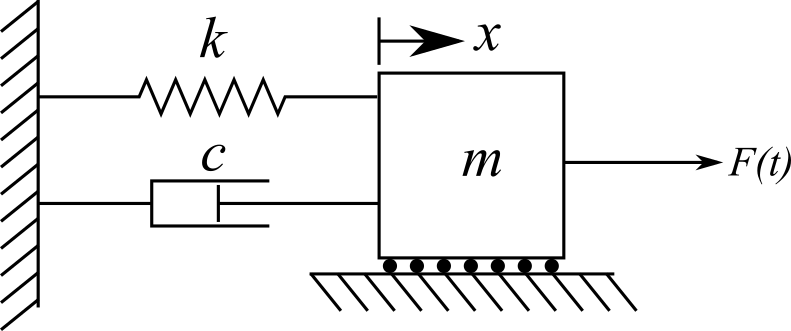
\includegraphics[width=0.4\textwidth]{../../Figures/forced_spring_mass_damper_system.png}
%\end{figure}
%that can be described the the EOM in standard form:
%\begin{equation}
%\ddot{x}(t) + 2 \zeta \omega_n \dot{x}+ \omega_n^2x(t) = 0 \text{, where }x(0)=x_0 \text{, and } \dot{x}(0) = v_0 
%\end{equation}
%Taking the Laplace transform of both sides of the EOM yields:
%\begin{equation}
%\big(s^2X(s) -sx_0 -v_0\big)+\big(s2 \zeta \omega_n X(s)-x_0\big)+\big(\omega_n^2X(s)\big) = 0
%\end{equation}
%considering that $sx_0 + x_0$ can be expressed as $sx_0$ because they are both based on the initial condition $x_0$. solving for the output of the system $X(s)$ yields:
%\begin{equation}
%X(s) = \frac{sx_0 + v_0}{s^2 + 2 \zeta \omega_n s+ \omega_n^2}
%\end{equation}
%Using the method of partial fractions, this can be expressed as inverse Laplace transform $x(t) = \Laplace{X(s)}^{-1}$ resulting in:
%\begin{equation}
%F(s) \text{ is } \frac{1}{s^2 + 2 \zeta \omega s+ \omega^2} \text{ when } f(t) \text{ is}\frac{1}{\omega_d}e^{-\zeta \omega t}\text{sin}(\omega_n t),
%\end{equation}
%\begin{equation}
%\text{when } \zeta < 1\text{, and } \omega_d = \sqrt{1-\zeta^2} \nonumber
%\end{equation}
%Therefore, we can obtain the solution for the system output $X(s)$ as:
%\begin{equation}
%x(t) = x_0 \text{cos}(\omega_n t) + \frac{v_0}{\omega_n}\text{sin}(\omega_n t)
%\end{equation}

\subsection*{Impulse Response Function}
A very common source of vibration is the sudden application for a short-duration force called an impulse. An impulse excitation is a force that is applied for a very short, or infinitesimal, length of time and represents one example of a shock loading. An impulse is a nonperiodic force that is represented by the symbol $\delta$. The response of a system to an impulse is identical to the free response of the system to certain initial conditions.This is illustrated in the following, in many useful situations the applied force $F(t)$ is impulsive in nature
(i.e., acts with large magnitude for a very short period of time).

\begin{figure}[H]
	\centering
	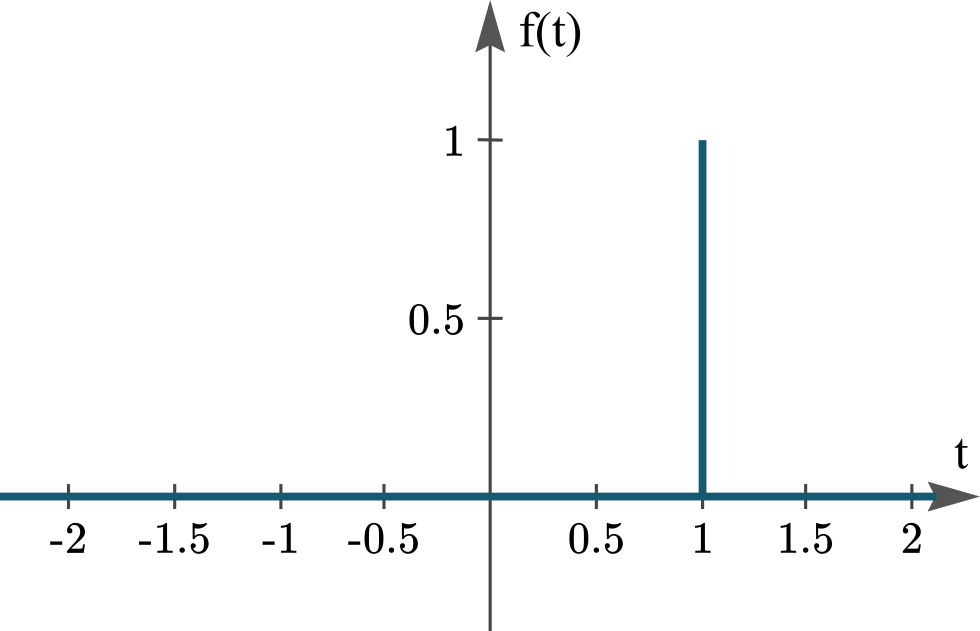
\includegraphics[width=0.5\textwidth]{../../Figures/impulse_time_history.png}
\end{figure}

The impulse response function can be solved for analytically, however, we will solve it using the transfer function approach. Here we will consider the under-damped spring-mass system. First, assume that the system is at rest (no initial conditions). Next, we write the EOM as:
\begin{equation}
m\ddot{x} +c\dot{x} +kx = \delta(t)
\end{equation}
Taking the Laplace transform of both sides of the equation yields 
\begin{equation}
m\big(s^2X(s)-sx(0) - \dot{x}(0)\big) + c\big(sX(s)-x(0)\big) +kX(s) =1
\end{equation}
However, \textbf{if we assume zero initial conditions} (a system at rest when the impulse happens), the equation simplifies to. 
\begin{equation}
ms^2X(s) + csX(s) +kX(s) =1
\end{equation}
or
\begin{equation}
(ms^2 + cs +k)X(s) =1
\end{equation}
note that the $\Laplace{\delta}=1$ per \#1 in the transform table. Solving this equation for $X(s)$:
\begin{equation}
X(s) = \frac{1}{m} \cdot \frac{1}{s^2 + 2 \zeta \omega_n s + \omega_n^2}
\end{equation}
Again, the mass is extracted to develop a formulation that can be found in the Laplace tables. Setting the constraint that $\zeta<1$ and consulting \#10 in the table for Laplace transforms results in:
\begin{equation}
x(t) = \frac{1}{m \omega_d} e^{-\zeta \omega_n t} \text{sin}(\omega_dt)
\end{equation}
where this is the general solution for a damped system subjected to an impulse loading function. For the undamped case a solution can be obtained by setting $\zeta=0$. This Results in the following form for the undamped case:
\begin{equation}
x(t) = \frac{1}{m \omega_n}\text{sin}(\omega_n t)
\end{equation}
Below is a typical response for both a undamped and underdamped 1-DOF system subject to an impulse response at $t=0$ seconds. 
\begin{figure}[H]
	\centering
	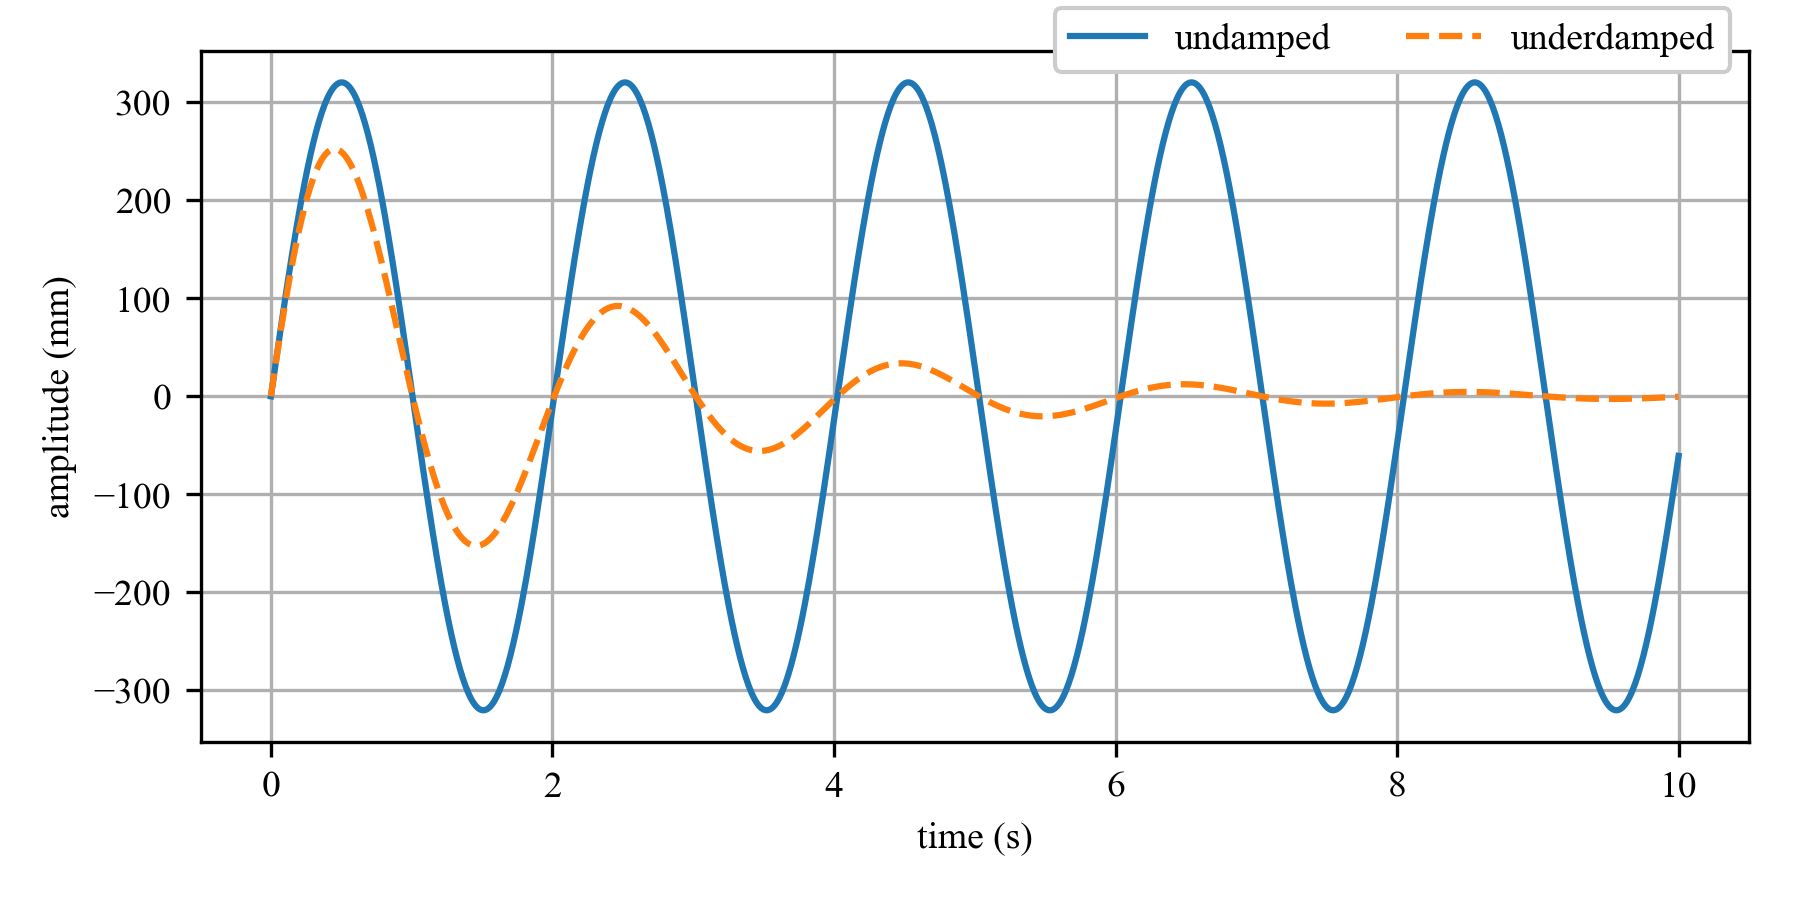
\includegraphics[width=0.75\textwidth]{../../Figures/response_impulse.png}
\end{figure}



\subsection*{Unit step function}
Now consider a unit step function $\Phi$: 

\begin{figure}[H]
	\centering
	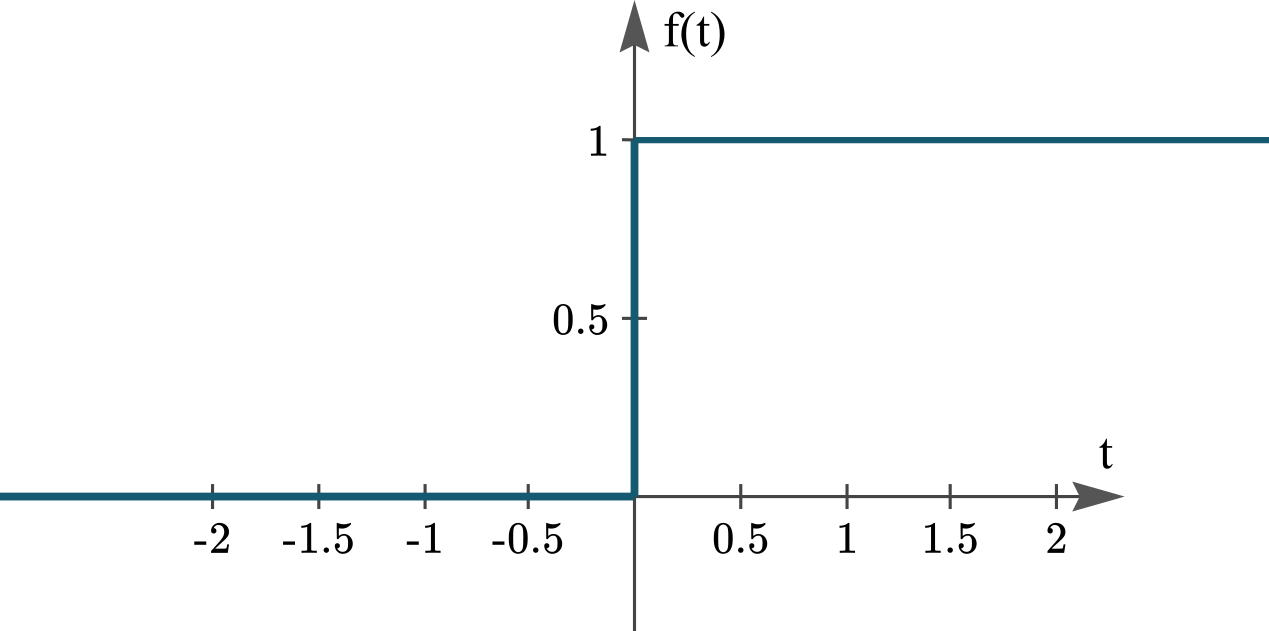
\includegraphics[width=0.5\textwidth]{../../Figures/unit_step_function.png}
\end{figure}

A step function is a common loading situation and can represent the dropping of a load into a truck, a car going over a curve, or a motor starting up. 


The Laplace transform of the function, for a unit step function $\Phi$, is: 
\begin{equation*}
\Laplace{\Phi(t)} = \int_{0}^{\infty} e^{-st}dt = -\frac{e^{-\infty}}{s} +\frac{e^{-0}}{s} =\frac{1}{s}
\end{equation*}
This also lines up with Laplace Transform \# 3 from the attached table. This would be expected as $\Phi$ is used to represent the unit step function (i.e. a step function with a displacement of 1). As we consider linear systems in this class, we can scale the magnitude of the response by the magnitude of the impulse after the transform is performed. 

\subsection*{Undamped spring-mass system}

For a spring-mass system subjected to a unit step, \textbf{assuming both initial conditions are zero}, the solution can be obtained using the transform method. First, the EOM is 
\begin{equation}
m\ddot{x}(t) + kx(t) = \Phi(t)
\end{equation}
Taking the Laplace transform of both sides and assuming zero initial conditions yields:
\begin{equation}
	ms^2X(s)+kX(s) =\frac{1}{s}
\end{equation}
Next, this equation is solved for $X(s)$ as:
\begin{equation}
	X(s) = \frac{1}{s(ms^2+k)}
\end{equation}
This can be rearranged as:
\begin{equation}
	X(s) = \frac{1}{m} \cdot \frac{1}{s(s^2+\omega_n^2)}
\end{equation}
where $\frac{1}{m}$ will pass through the Laplace function. Therefore, taking the inverse Laplace transform yields:
\begin{equation}
	x(t) = \frac{1}{m} \cdot \frac{1}{\omega_n^2}\big(1-\text{cos}(\omega_n t)\big) = \frac{1}{k}\big(1-\text{cos}(\omega_n t)\big)
\end{equation}
 
\subsection*{Under damped spring-mass system}

For a spring-mass-damper system subjected to a unit step, assuming both initial conditions are zero, the solution can be obtained using the transform method. First, the EOM is:
\begin{equation}
m\ddot{x}(t) + c\dot{x} + kx(t) = \Phi(t)
\end{equation}
Converting to the standard form results in:
\begin{equation}
\ddot{x}(t) + 2  \zeta \omega_n\dot{x} + \omega_n^2x(t) = \frac{1}{m} \cdot \Phi(t)
\end{equation}
taking the Laplace transform of both sides and assuming zero initial conditions yields:
\begin{equation}
	s^2X(s) + 2  \zeta \omega_n s X(s) + \omega_n^2 X(s)  =\frac{1}{m} \cdot \frac{1}{s}
\end{equation}
Next, this equation is solved for $X(s)$ as:
\begin{equation}
	X(s) = \frac{1}{s^2 + 2  \zeta \omega_n s + \omega_n^2} \cdot \frac{1}{m} \cdot \frac{1}{s}
\end{equation}
multiplying the right-hand-side of this equation by  $\frac{\omega_n^2}{\omega_n^2}$ results in:
\begin{equation}
	X(s) = \frac{1}{m \omega_n^2} \cdot \frac{\omega_n^2}{s(s^2+2\zeta\omega_n s+\omega_n^2)}
\end{equation}
Again, the $\frac{1}{m\omega_n^2}$ will pass through the Laplace function. Therefore, taking the inverse Laplace transform yields:
\begin{equation}
	x(t) = \frac{1}{m \omega_n^2} \cdot \Big(1 - \frac{\omega_n}{\omega_d}e^{-\zeta \omega_n t}\text{sin}(\omega_dt + \phi)\Big)\text{, where } \phi = \text{cos}^{-1}(\zeta)\text{, where } \zeta<1
\end{equation}
After obtaining equations for the undamped and under damped cases, the responses for the unit step, solved with the transform method, can be plotted as:
\begin{figure}[H]
	\centering
	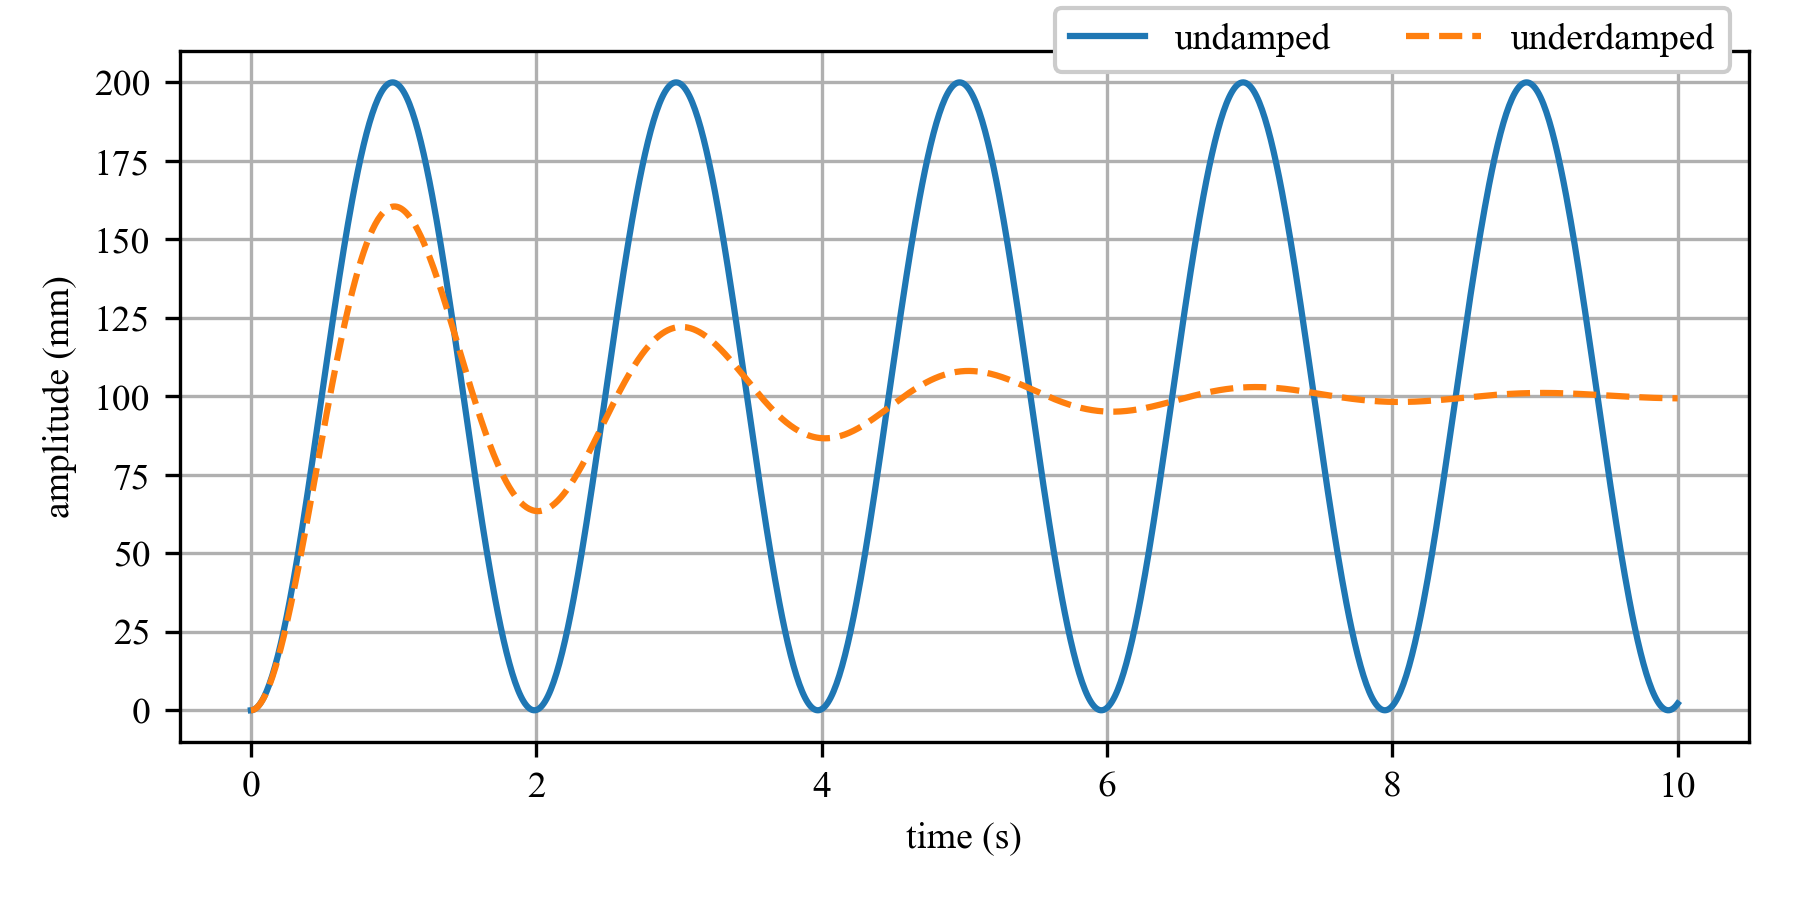
\includegraphics[width=0.75\textwidth]{../../Figures/unit_step.png}
\end{figure}
Note that the system will settle out around $F_0/k$ where $F_0  \Phi$ is a scaling factor for the step loading.

\pagebreak

\textbf{Example 1}

A load of dirt of mass $m_d$ is dropped on the floor of a truck bed.The truck bed is modeled as a spring-mass-damper system (of values $k$, $m$, and $c$, respectively).The load is
modeled as a force $F(t) = m_dg$ applied to the spring-mass-damper system, as illustrated
in the following figure. This allows a crude analysis of the response of the truck's suspension. First assume that the trucks damper is broken, how does the maximum dynamic displacement compare to the static displacement. What would happen to the maximum displacement if the damper was repaired on the truck? %Next, using a damping value of $\zeta=0.5$ and $\omega_n=\pi$ what is the maximum displacement. How does this compare to the displacement for the case without the damper?  

\begin{figure}[H]
	\centering
	\includegraphics[width=0.8\textwidth]{../../Figures/dump_truck.png}
\end{figure}

\textbf{Solution }

First, setting the load applied to the truck as 1 unit, it can be seen that this is a unit step loading condition and a broken damper represents an undamped case. To obtain a rough idea about the nature of static and dynamic displacement, the undamped displacement is

\begin{equation}
	x(t) = \frac{1}{k}\big(1-\text{cos}(\omega_n t)\big) = \frac{m_dg}{k}\big(1-\text{cos}(\omega_n t)\big)
\end{equation}
 
This equation has a maximum amplitude when the cos$(\omega_dt)=-1$, resulting in:
\begin{equation}
	x(t) = \frac{m_dg}{k}\big(1-(-1)\big)
\end{equation}
This can be rearranged for the maximum displacement value $x_\text{max} $ as:
\begin{equation}
	x_\text{max} = 2\frac{m_dg}{k}
\end{equation} 
This is twice the static displacement (i.e., twice the distance the truck would be deflected if the dirt were placed gently and slowly onto it). Thus, if the truck were designed with springs based only on the static load, with no margins of safety, the springs in the truck
would potentially break, or permanently deform, when subjected to the same mass applied dynamically (e.g., dropped) into the truck. Hence, it is important to consider the vibration (dynamic) response in designing structures that could experience dynamic loading.

%\textbf{Example 1 - under damped}
%For the case where the truck has a damper with a value of $\zeta=0.5$, the displacement $(x)$ can be modeled as:
%\begin{equation}
%	x(t) = \frac{m_dg}{m \omega_n^2} \cdot \Big(1 - \frac{\omega_n}{\omega_d}e^{-\zeta \omega_n t}\text{sin}(\omega_dt + \phi)\Big)\text{, where } \phi = \text{cos}^{-1}(\zeta)
%\end{equation}


\textbf{Example 2}

In testing, an hammer is used to excite a 1-DOF system with an impact (i.e. impulse), however, the hammer ascendantly impacts the system twice. The first impact has a force of 0.2 N, while the second has a force of 0.1 N and happens 0.1 seconds after the first impact. Plot the response for the double impact. The system has the parameters $m$ = 1 kg, $c$ = 0.5 kg/s, k = 4 N/m. 

\textbf{Solution }

First, we can define the forcing function as:

\begin{equation}
	F(t) = 0.2 \delta (t) + 0.1 \delta(t-\tau)
\end{equation}
where $\tau$ is the offset between the first and second impacts. Next, considering that the unit impulse has a magnitude of 1 we can obtain solutions for the first impact by first writing it's EOM:

\begin{equation}
m\ddot{x} +c\dot{x} +kx =0.2 \delta(t)
\end{equation}
Taking the Laplace transform of both sides of the equation yields 
\begin{equation}
m\big(s^2X(s)-sx(0) - \dot{x}(0)\big) + c\big(sX(s)-x(0)\big) +kX(s) = 0.2
\end{equation}
However, assuming zero initial conditions, the equation simplifies to. 
\begin{equation}
(ms^2 + cs +k)X(s) = 0.2
\end{equation}
Solving this equation for $X(s)$:
\begin{equation}
X(s) = \frac{0.2}{m} \cdot \frac{1}{s^2 + 2 \zeta \omega_n s + \omega_n^2}
\end{equation}
Again, consulting \#10 in the table for Laplace transforms results in:
\begin{equation}
x_1(t) = \frac{0.2}{m \omega_d} e^{-\zeta \omega_n t} \text{sin}(\omega_dt)
\end{equation}
where this is the general solution for a damped system subjected to an impulse loading function. The second impact can now be solved for using the same method. However, now the time $(t)$ must be offset by $(\tau)$ to allow the impact to still be located at $t=0$ in terms of the second impact. This results in:
\begin{equation}
	x_1(t) = \frac{0.2}{m \omega_d} e^{-\zeta \omega_n t} \text{sin}(\omega_dt)
\end{equation}
\begin{equation}
	x_2(t) = \frac{0.1}{m \omega_d} e^{-\zeta \omega_n (t-\tau)} \text{sin}\big(\omega_d(t-\tau)\big)
\end{equation}
Next, using the knowledge that the systems are linear and that the Laplace transform of a linear combination of two transforms is the same as the linear transformation of these functions we can build the piecewise function:

\[
  x(t) = x_1(t) + x_2(t) =
  \begin{cases}
\frac{0.2}{m \omega_d} e^{-\zeta \omega_n t} \text{sin}(\omega_dt) & \text{if } t < \tau \\
\frac{0.2}{m \omega_d} e^{-\zeta \omega_n t} \text{sin}(\omega_dt)  + \frac{0.1}{m \omega_d} e^{-\zeta \omega_n (t-\tau)} \text{sin}(\omega_d(t-\tau) & \text{if } \tau \leq t 
  \end{cases}
\]


For the mass, damping, and stiffness values given above this can be plotted as:
\begin{figure}[H]
	\centering
	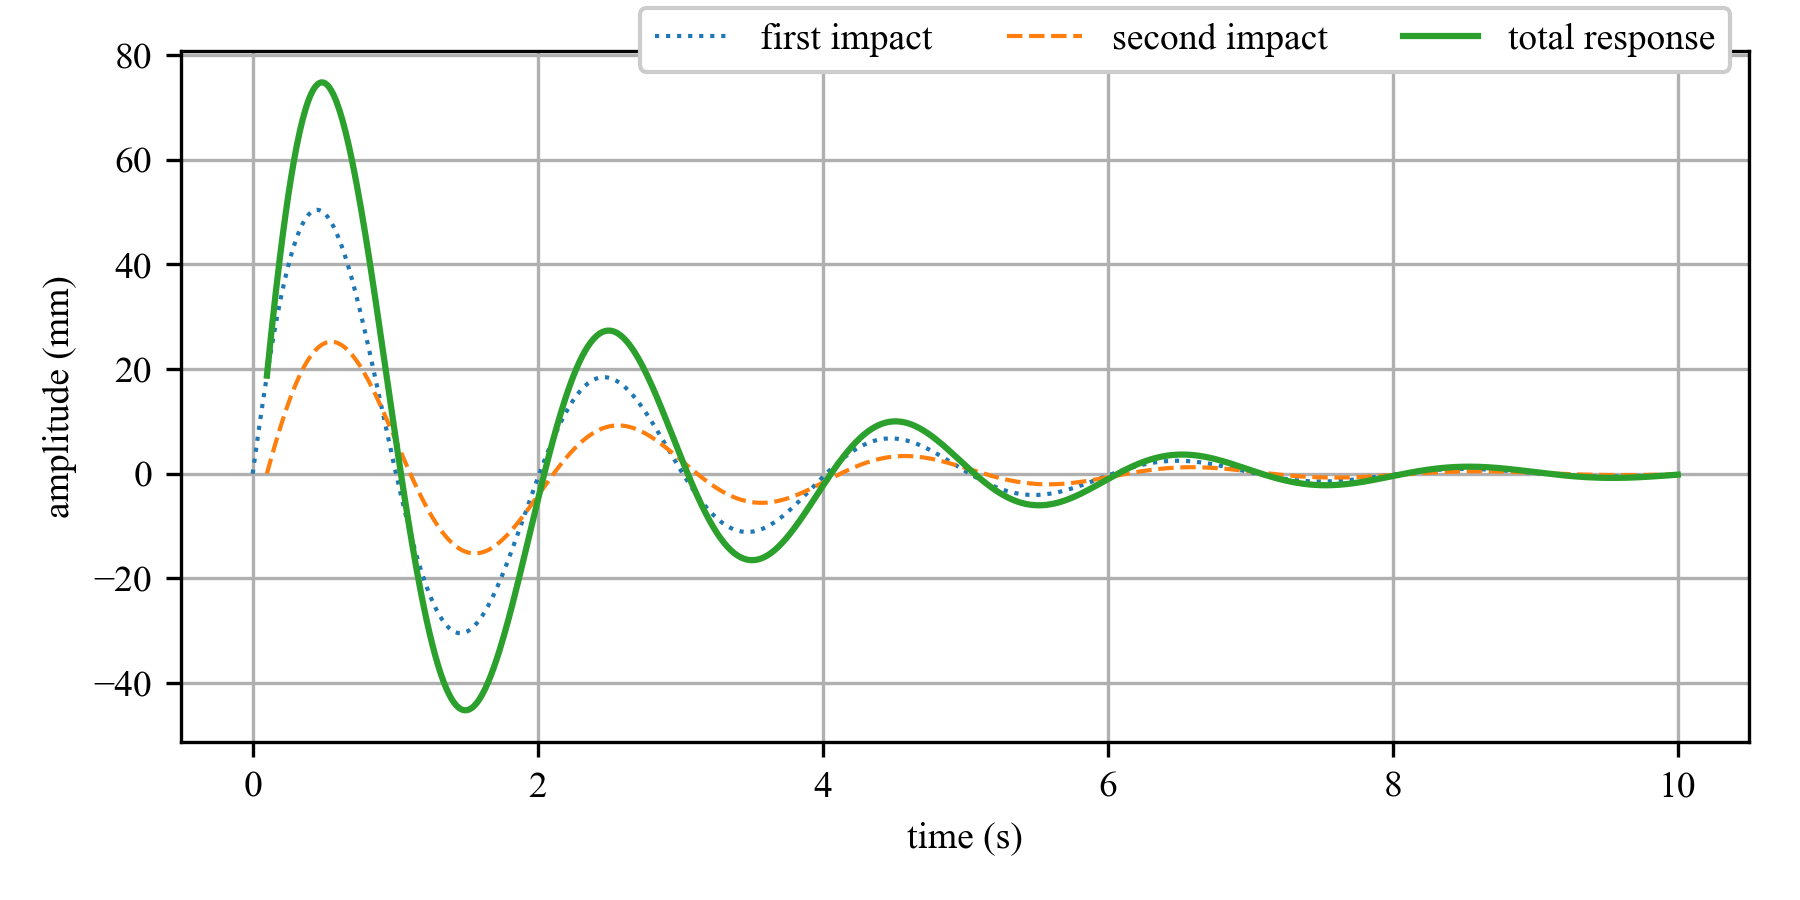
\includegraphics[width=0.75\textwidth]{../../Figures/response_double_impact.png}
\end{figure}






\newpage




\pagestyle{empty}
\vspace{-20ex}
\begin{center}
{\large{}\textbf{Table of Laplace Transforms for Vibrations}} \\
\normalsize{} This is a partial lists of important Laplace transforms for vibrations that assumes \\ zero initial conditions, $0 < t$, and $\zeta < 1$.
\end{center}

\vspace{0ex}
{\small
\renewcommand{\arraystretch}{1.5}
\begin{multicols}{2}
\begin{center}
\begin{tabbing}
\hspace*{1.5 in}\=\hspace{1.5in}\= \kill
	$f(t)$ \> $\Laplace{f(t)}=F(s)$ \> \\ \noindent\rule{8.0cm}{0.4pt} \\
	$\delta(t)$	\> 1 \> \LTNUM \\ \\
	$\delta(t-t_0)$ \> $e^{-st_0}$ \>\LTNUM \\ \\
	$1$       			 \> $\dfrac{1}{s}$           \>\LTNUM \\ \\
	$e^{at}$ 	\> $\dfrac{1}{s-a}$ 	\>\LTNUM \\ \\
	$\sin (\omega t) $ 	\> $\dfrac{\omega}{s^2+\omega^2}$ \>\LTNUM \\ \\
	$\cos (\omega t) $ 	\> $\dfrac{s}{s^2+\omega^2}$ \>\LTNUM \\ \\
	
	$\sinh (\omega t) $	\> $\dfrac{\omega}{s^2-\omega^2}$ \>\LTNUM \\ \\
	$\cosh (\omega t) $	\> $\dfrac{s}{s^2-\omega^2}$ \>\LTNUM \\ \\
	$\dfrac{1}{\omega^2}\big(1-\cos(\omega t)\big)$ \> $\dfrac{1}{s(s^2+\omega^2)}$ \>\LTNUM \\ \\
	$\dfrac{1}{\omega_d}e^{-\zeta \omega t}\sin(\omega_d t)$ \> $\dfrac{1}{s^2+2\zeta \omega s+\omega^2}$ \>\LTNUM \\ \\
	$1-\dfrac{\omega}{\omega_d}e^{-\zeta \omega t}\sin(\omega_d t + \phi)$, $\phi =\cos^{-1}(\zeta) \dots $ \\ \> $\dfrac{\omega^2}{s(s^2+2\zeta \omega s+\omega^2)}$ \>\LTNUM \\ \\
	$\dfrac{t^{n-1}}{(n-1)!}$, $ n=1,2,\dots $ \> $\dfrac{1}{s^n}$ \>\LTNUM \\ \\
	$t^n $, $n=1,2,\dots$     \> $\dfrac{n!}{s^{n+1}}$    \>\LTNUM \\ \\
	$t^ne^{\omega t}$, $ n=1,2,\dots $	\> $\dfrac{n!}{(s-\omega)^{n+1}}$	\>\LTNUM \\ \\
	$\dfrac{1}{\omega}(1-e^{-\omega t}) $	\> $\dfrac{1}{s(s+\omega)}$	\>\LTNUM \\ \\
	$\dfrac{1}{\omega^2}(e^{-\omega t}+\omega t - 1) $	\> $\dfrac{1}{s^2(s+\omega)}$	\>\LTNUM \\ \\
\end{tabbing}
\end{center}

\columnbreak

\begin{center}
\begin{tabbing}
\hspace*{1.5in}\=\hspace{1.5in}\= \kill
	$f(t)$ \> $\Laplace{f(t)}=F(s)$ \> \\ \noindent\rule{8.0cm}{0.4pt} \\
	$\dfrac{1}{\omega^3}\big(\omega t - \sin(\omega t)\big) $	\> $\dfrac{1}{s^2(s^2+\omega^2)}$	\>\LTNUM \\ \\
	$\dfrac{1}{2\omega^3}\big(\sin(\omega t) - \omega t \cos(\omega t)\big) \dots $	\\ \> $\dfrac{1}{(s^2+\omega^2)^2}$	\>\LTNUM \\ \\
	$\dfrac{t}{2\omega} \sin(\omega t)$	 \> $\dfrac{s}{(s^2+\omega^2)^2}$	\>\LTNUM \\ \\
	$t\sin (\omega t) $  	\> $\dfrac{2\omega s}{(s^2+\omega^2)^2}$ \>\LTNUM \\ \\
	$t\cos (\omega t) $  	\> $\dfrac{s^2-\omega^2}{(s^2+\omega^2)^2}$ \>\LTNUM \\ \\
	$e^{at}\sin (\omega t) $	\> $\dfrac{\omega}{(s-a)^2+\omega^2}$  \>\LTNUM \\ \\
	$e^{at}\cos (\omega t) $	\> $\dfrac{s-a}{(s-a)^2+\omega^2}$  \>\LTNUM \\ \\
	$e^{at}\sinh (\omega t) $	\> $\dfrac{\omega}{(s-a)^2-\omega^2}$  \>\LTNUM \\ \\
	$e^{at}\cosh (\omega t) $	\> $\dfrac{s-a}{(s-a)^2-\omega^2}$  \>\LTNUM \\ \\
	$\dfrac{1}{\omega_2}\sin(\omega_2 t) - \dfrac{1}{\omega_1}\sin (\omega_1 t) \dots $	 \\ \> $\dfrac{\omega_1^2-\omega_2^2}{(s^2+\omega_1^2)(s^2+\omega_2^2)}$	\>\LTNUM \\ \\
	$\cos(\omega_2 t) - \cos (\omega_1 t)  $	\> $\dfrac{s(\omega_1^2-\omega_2^2)}{(s^2+\omega_1^2)(s^2+\omega_2^2)}$	\>\LTNUM \\ \\
	$e^{at}f(t)$	\> $F(s-a)$	\>\LTNUM \\ \\ 
	$f(t-a)\Phi(t-a)$ \> $e^{-as}F(s)$ \>\LTNUM \\ \\
	$\Phi(t-a)$ \> $\dfrac{e^{-as}}{s}$ \>\LTNUM \\ \\
	$f'(t)$ 	\> $sF(s) - f(0)$ \>\LTNUM \\ \\
\end{tabbing}
\end{center}
\end{multicols}
}

% Unused Laplace Transforms
%$f^{n}(t)$ 	\> $s^nF(s) - s^{(n-1)} f(0) - $ \\ \\
% \> $\cdots - f^{(n-1)}(0)$ \>\LTNUM \\ \\
%$\displaystyle{\int_0^t f(x)g(t-x)dx}$ \> $F(s)G(s)$ \>\LTNUM \\ \\
%
%$t^x$ ($x\geq-1\in\mathbb{R}$)     \> $\dfrac{\Gamma(x+1)}{s^{x+1}}$ \>\LTNUM\\ \\
%
%$\dfrac{e^{at}-e^{bt}}{a-b}$	\> $\dfrac{1}{(s-a)(s-b)}$ \>\LTNUM\\ \\ 
%$f(t)$ \> $\Laplace{f(t)}=F(s)$ \> \\ \\
%$\dfrac{ae^{at}-be^{bt}}{a-b}$	\> $\dfrac{s}{(s-a)(s-b)}$ \>\LTNUM\\ \\ 
%$te^{at}$	\> $\dfrac{1}{(s-a)^2}$	\>\LTNUM \\ \\
%$t\sinh (\omega t) $  	\> $\dfrac{2\omega s}{(s^2-\omega^2)^2}$ \>\LTNUM \\ \\
%$t\cosh (\omega t) $  	\> $\dfrac{s^2+\omega^2}{(s^2-\omega^2)^2}$ \>\LTNUM \\ \\
%$\dfrac{\sin (at)}{t}$	\> $\arctan \dfrac{a}{s}$ \>\LTNUM \\ \\
%$\dfrac{1}{\sqrt{\pi t}}e^{-a^2/4t}$	\> $\dfrac{e^{-a\sqrt{s}}}{\sqrt{s}}$ \> \LTNUM \\ \\
%$\dfrac{a}{2\sqrt{\pi t^3}}e^{-a^2/4t}$	\> $e^{-a\sqrt{s}}$ \> \LTNUM \\ \\
%$\text{erfc}\left(\dfrac{a}{2\sqrt{t}}\right)$ \>  $\dfrac{e^{-a\sqrt{s}}}{s}$ \> \LTNUM \\ \\
% $t^nf(t)$ 	\> $(-1)^n\dfrac{d^nF(s)}{ds^n}$  \>\LTNUM \\ \\
%{\tiny \textcopyright  2011 B.E.Shapiro for \href{http://integral-table.com}{integral-table.com}. This work is licensed under a} \\

%{\tiny\href{http://creativecommons.org/licenses/by-nc-sa/3.0/}{Creative Commons Attribution-NonCommercial-ShareAlike 3.0 Unported License}. } 

\end{document}


























